\documentclass[tikz,border=2mm]{standalone}

\newcommand\twodigit[1]{\expandafter\twodigitaux#1\relax}
\def\twodigitaux#1.#2\relax{\ifnum10>#1\relax0\fi\pgfmathprintnumber{#1.#2}}

% syntax: \drawtimeline{starthour}{startmin}{endhour}{endmin}{interval}
\newcommand{\drawtimeline}[6]{%
    \pgfmathsetmacro\Start{#1*60+#2}
    \pgfmathsetmacro\End{#3*60+#4}
    \pgfmathsetmacro\Span{\End-\Start}
    \pgfmathsetmacro\NumLabels{\Span/#5}
    \pgfmathsetmacro\Labels{#6/\NumLabels}
    \pgfmathsetmacro\Ticks{#6/\Span}
        % draw line
        \draw [thick](0,0) -- (#6,0);
        % draw small ticks
        \foreach \y  in {0,1,..., \Span} {%
            \draw[thin, yshift=0pt, xshift=\Ticks*\y] (0pt,+2pt) -- (0pt,-2pt);}
        % draw big ticks and labels
        \foreach \y  
            [evaluate=\y as \hrs using ({div(\y*#5+\Start,60)}] 
            [evaluate=\y as \mns using ({mod(\y*#5+\Start,60)}]
                in {0,1,...,\NumLabels} {% 
                    \draw[yshift=-3ex, xshift=\Labels*\y] node[below]{%
                        $\pgfmathprintnumber{\hrs}$:%
                        $\twodigit{\mns}$};
                    \draw[thick, yshift=0pt, xshift=\Labels*\y] (0pt,+5pt) -- (0pt,-5pt);}
}%


\begin{document}
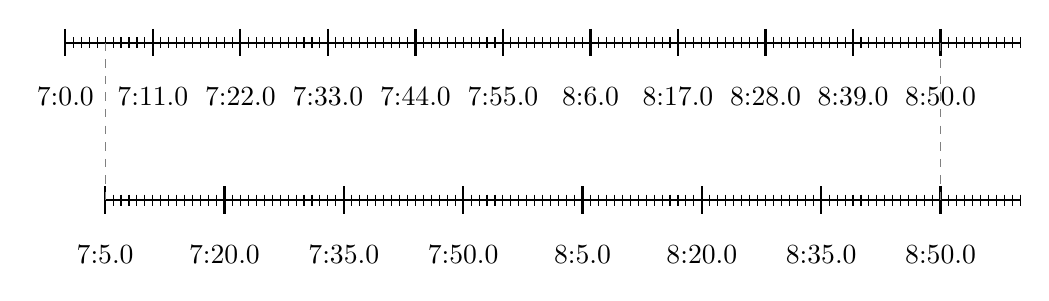
\begin{tikzpicture}% would be nice to make the shifts automatic
\begin{scope}% 345pt standard textwidth
    \drawtimeline{7}{00}{9}{00}{11}{345pt}
\end{scope}
\begin{scope}[shift={(14.37pt,-2cm)}]% 330.63=345-14.37
    \drawtimeline{7}{05}{9}{00}{15}{330.63pt}
\end{scope}
\draw[dashed,gray] (14.37pt,0) -- (14.37pt,-2cm) {};
\draw[dashed,gray] (316.25pt,0) -- (316.25pt,-2cm) {};
\end{tikzpicture}
\end{document}


